\documentclass[conference]{IEEEtran}
\IEEEoverridecommandlockouts
\usepackage{amsmath,amssymb,amsfonts}
\usepackage{algorithmic}
\usepackage{graphicx}
\usepackage{textcomp}
\usepackage{xcolor}
\usepackage{listings}
\usepackage{float}
\usepackage{array}
\usepackage{url}
\usepackage{booktabs}
\def\BibTeX{{\rm B\kern-.05em{\sc i\kern-.025em b}\kern-.08em
    T\kern-.1667em\lower.7ex\hbox{E}\kern-.125emX}}
\lstset{
    basicstyle=\ttfamily\scriptsize,
    breaklines=true,
    frame=single,
    keywordstyle=\color{blue},
    commentstyle=\color{gray},
    stringstyle=\color{teal},
    xleftmargin=4pt,
    xrightmargin=4pt,
}

\usepackage[style=numeric,sorting=none,backend=biber]{biblatex}
\addbibresource{refs.bib}

\begin{document}

\title{Entropy-Based Dynamic Routing for Energy Efficient Spiking Neural Networks}
% have title indicate same architecture SNNs not just the "routing" idea. 

\author{
    \IEEEauthorblockN{
        Gaurav Gupta,
        Laurena Chen,
        Kevin Nguyen,
        Meghana Reddy,
        Jason Eshraghian
    }
    \IEEEauthorblockA{
        \textit{University of California, Santa Cruz,
        Santa Cruz, CA 95064 USA}
    }
}

\maketitle

\begin{abstract}
Spiking neural networks (SNNs) are machine learning models that provide low energy inference. However, using a single SNN on both simple and complex input data might not be the most energy efficient approach. We introduce an entropy based routing framework that dynamically selects between sparse and dense SNN models based on input temporal structure. Low complexity inputs are routed to a sparse SNN with reduced spiking activity and lower energy cost; high complexity inputs are routed to a dense SNN with higher capacity. We obtain a routing metric using Lempel Ziv Complexity (LZC) and measure its computational cost directly on an STM32 microcontroller and SynSense Xylo hardware to assess real world routing overhead. The routing threshold is optimized using ROC analysis and geometric mean criteria. Lastly, we validate this approach on three distinct datasets, DVSGesture, Spiking Heidelberg Digits (SHD), and UCI HAR.

\end{abstract}

\begin{IEEEkeywords}
Spiking neural networks, neuromorphic computing, Lempel Ziv complexity, transition count, entropy based routing, energy efficient computation
\end{IEEEkeywords}

% ---------------------------------------------------------------
\section{Introduction}
% ---------------------------------------------------------------

Energy efficiency is a central challenge in edge AI. Spiking neural networks (SNNs) have emerged as a promising approach to low power inference because they communicate through sparse, event driven spikes rather than dense, continuous activations. On neuromorphic hardware platforms such as Intel Loihi, IBM TrueNorth, SpiNNaker, and SynSense Xylo, this property enables energy efficient processing of continuous sensory streams like audio, video, and IMU signals at a fraction of the power required by conventional deep learning systems \cite{davies2018loihi, akopyan2015truenorth, furber2014spinnaker, gallego2022eventVision}.

However, one limitation of SNN deployments is that a single model cannot be both energy efficient and accurate across inputs of varying complexity. Real world sensory data varies widely in difficulty. Event based datasets like DVSGesture and SHD contain both simple, low entropy inputs—slow repetitive gestures, steady tones—and complex, high entropy ones with rapid temporal transitions. Sensor streams like UCI HAR range from smooth, predictable activities like walking to more erratic patterns. A fixed size SNN is forced to make an uncomfortable trade off: large models handle complex inputs well but waste energy on easy ones; small models are efficient but often fail on harder inputs.

Mixture of Experts (MoE) approaches address this by training multiple models and selecting between them per input. However, standard MoE methods for SNNs typically require separate training pipelines and distinct parameter sets for each model, increasing storage and deployment complexity. We take a simpler approach: use a single SNN architecture and produce sparse and dense variants by adjusting only the neuron level parameters such as the membrane time constant ($\tau_{mem}$), spike threshold, and spike regularization strength. The sparse variant fires less and consumes less energy; the dense variant fires more freely and achieves higher accuracy. This assumes that routing between the two models requires only a lightweight complexity estimate of each input.

For routing, we evaluate two complexity metrics. The first is Lempel Ziv Complexity (LZC), which estimates the diversity of patterns in a spike sequence and is widely used in neural signal analysis \cite{amigo2004entropySNN}. The second is Transition Count (TC), which simply counts the number of $0{\to}1$ and $1{\to}0$ transitions in the binarized spike sequence, which is a linear time operation requiring no data structures. We hypothesized that TC, despite its simplicity, might capture enough complexity information for routing while being far cheaper to compute.

A key contribution of this work is directly measuring the computational cost of both routing metrics on embedded hardware. We implemented both LZC and TC in C and ran them on an STM32 microcontroller, using the ARM hardware cycle counter to record exact cycle counts per sample. These were projected to energy using the power specification of the low power STM32L476 (180 pJ/cycle). This allowed us to compare routing overhead against actual SNN inference energy on Xylo hardware, and ask whether routing can ever pay for itself in practice.

Our results show that LZC is prohibitively expensive as a routing signal—costing hundreds to thousands of $\mu$J per sample on embedded hardware, far exceeding the SNN inference cost. TC, by contrast, costs only 7--9~$\mu$J per sample and achieves a stronger correlation with input complexity ($r > 0.99$), making it a significantly more viable candidate for real time neuromorphic routing. While even TC does not yet produce net energy savings in our current CPU based pipeline, it points toward a practical path forward: lightweight, linear time metrics that could eventually be implemented on chip.

In this work, we present a complete routing pipeline that: (1) computes input complexity using LZC or TC, (2) selects an optimal routing threshold via ROC analysis and G mean optimization, (3) routes each sample to the appropriate SNN variant, and (4) measures end to end accuracy and energy consumption. We validate this across DVSGesture (11 gesture classes), SHD (20 spoken digits), and UCI HAR (6 activity classes), combining Xylo hardware measurements with spike count based energy estimates.

% ---------------------------------------------------------------
\section{Background}
% ---------------------------------------------------------------

\subsection{Spiking Neural Networks}

SNNs process information through discrete, temporally precise spikes rather than continuous activations. Neurons integrate incoming spikes into a membrane potential and fire only when that potential exceeds a threshold—after which it resets. This event driven mechanism means neurons are silent most of the time, which is the primary source of SNN energy efficiency \cite{rieke1997spikes, maass1997thirdgen}. Unlike ANNs, which perform dense matrix multiplications at every layer on every forward pass, SNNs only require computation when a spike happens \cite{rueckauer2017conversionSNN}.

On neuromorphic hardware like Intel Loihi, IBM TrueNorth, and SynSense Xylo, this translates directly to lower power consumption: energy is spent only on active synaptic events, not on idle processing \cite{davies2018loihi, akopyan2015truenorth}. SNNs are particularly well suited to temporal data such as audio, event based video, and IMU signals, which arrive as streams of events rather than static frames.

Energy in SNNs is typically estimated using spike counts as a proxy—each spike triggers a fixed number of synaptic operations, so total spike activity is a good enough estimation of energy consumption \cite{maass1997thirdgen}. On hardware platforms, energy can also be measured directly using on chip monitors or external instrumentation \cite{akopyan2015truenorth}.

\subsection{Entropy and Complexity Measures for Spike Trains}

Binary data streams, also known as spike trains, can be characterized by entropy and complexity metrics that capture how predictable or structured the temporal activity is. LZC estimates the number of distinct patterns in a binary sequence by tracking how many unique subsequences are needed to represent it. It has been widely applied in neuroscience and biomedical signal analysis as a measure of temporal irregularity \cite{amigo2004entropySNN}. Other complexity measures—sample entropy, approximate entropy, permutation entropy—have similarly been used to characterize neural, cardiac, and EEG signals \cite{nicolaou2012eeg, costa2002multiscaleEntropy, pincus1991approxEntropy}.

Despite their utility for characterizing neural data, these entropy measures have rarely been used make model selection for multiple SNN pipelines. This work explores whether complexity metrics can serve as lightweight routing signals, and specifically whether simpler metrics like Transition Count can match the routing quality of LZC.

\subsection{Computational Cost and Energy in SNNs}

SNN energy scales with spike activity rather than model size \cite{maass1997thirdgen}. Each spike produces a fixed set of synaptic operations, so reducing the firing rate directly reduces energy. Sparse models, which fire less frequently due to higher thresholds and stronger regularization, are therefore cheaper to run at the expense of low accuracy on complex inputs. This motivates the use of input adaptive routing: running a sparse model when spikes are sufficient, and falling back to a dense model when more representational capacity is needed \cite{teerapittayanon2016branchynet}.

% ---------------------------------------------------------------
\section{Methods}
% ---------------------------------------------------------------

\subsection{Datasets}

\paragraph*{DVSGesture}
The DVS128 Gesture dataset contains 11 human gesture classes captured with a 128$\times$128 dynamic vision sensor. Each sample is an event stream of polarity coded spikes at microsecond resolution. We convert each recording into a fixed length tensor of $T$ frames (typically 60-80), with positive and negative polarity channels kept separate, giving a \texttt{(2, H, W)} representation per frame. We follow the standard preprocessing pipeline from the public snnTorch implementation \cite{dlarionov2021dvsgesture}.

\paragraph*{SHD}
The Spiking Heidelberg Digits dataset contains 20 spoken digits encoded as spike trains across 700 frequency channels using a neuromorphic cochlea model. Each sample is converted to $T$ fixed frames by accumulating spikes within uniform time bins, producing a binary vector of length 700 per frame. No filtering or augmentation is applied beyond time binning.

\paragraph*{UCI HAR}
The UCI Human Activity Recognition dataset contains six activity classes (walking, walking upstairs, walking downstairs, sitting, standing, laying) recorded from smartphone accelerometer and gyroscope sensors. Each sample is a fixed length window of $T=128$ timesteps with 9 sensor channels (tri axial accelerometer, gyroscope, and body motion components) at 50~Hz. Samples are normalized per sample using z-score normalization.

\subsection{Entropy Metrics}

\subsubsection{LempelZiv Complexity}

LZC quantifies the number of distinct subsequences in a binary sequence—equivalently, how many unique patterns are needed to describe it. Higher LZC indicates more irregular, less compressible temporal structure. For each input sample, we flatten the spike tensor into a single binary string and compute LZC using the standard algorithm \cite{besson2016lzpython}:

\begin{lstlisting}[language=Python]
def lzcomplexity(ss):
    ii = 0; kk = 1; el = 1
    kmax = 1; cc = 1; nn = len(ss)
    while True:
        if ss[ii + kk - 1] == ss[el + kk - 1]:
            kk += 1
            if (el + kk) > nn:
                cc += 1; break
        else:
            if kk > kmax: kmax = kk
            ii += 1
            if ii == el:
                cc += 1; el += kmax
                if (el + 1) > nn: break
                ii = 0; kk = 1; kmax = 1
            else:
                kk = 1
    return cc
\end{lstlisting}

\subsubsection{Transition Count}

TC counts the number of $0{\to}1$ and $1{\to}0$ transitions in the binarized spike sequence. It is an $O(N)$ operation requiring a single linear pass with no data structures:

\begin{lstlisting}[language=C]
int transition_count(const int *events, int n) {
    int count = 0;
    for (int i = 1; i < n; i++)
        if (events[i] != events[i-1]) ++count;
    return count;
}
\end{lstlisting}

TC captures a simpler notion of complexity—how often the spike signal switches state—without the overhead of LZC's pattern dictionary. We include it as a potential low cost alternative routing signal.

\subsection{Entropy Based Data Splitting}

Routing decisions are made entirely on the held out test set to prevent information leakage. For each test sample, we compute a complexity score (LZC or TC) and assign a binary label: does the dense model succeed where the sparse model fails? We sweep candidate thresholds across the observed complexity range, compute a ROC curve, and select the threshold that maximizes the geometric mean (G mean) of sensitivity and specificity \cite{teerapittayanon2016branchynet, smetek2017thresholdROC, yang2020energyawareCascade}.


\subsection{Model Energy and Latency Measurement}

For UCI HAR, we deployed our own models on SynSense Xylo Audio 3 neuromorphic hardware and collected both energy and latency measurements directly from the board, sample-by-sample. This allows us to report the exact values for the energy and latency distributions. Routing decisions for the Xylo experiments used precomputed per-sample LZC values and cycle counts stored in an external file generated from the STM32 measurements. The samples were kept in fixed order during dataset loading, so the LZC row index matched the corresponding Xylo inference sample index exactly. Thus, Xylo energy and latency were measured on hardware, while routing complexity was reused from the earlier STM32 profiling run.

For DVSGesture and SHD, the datasets exceed the input constraints of the neuromorphic hardware, so we used energy estimation instead. We calibrated our energy estimates by training a baseline model that matches the architecture and hyperparameters from published papers that tested these datasets on neuromorphic hardware. We measured spike counts from this baseline model and divided by the reported average energy per inference to derive an energy per spike constant. We then applied this constant to our sparse and dense model spike counts to estimate their energy consumption. Note that it is important for us to copy the paper's model architecture for our sparse and dense models to ensure the most accurate energy estimate.

\subsection{SNN Model Architecture}

\paragraph*{UCI HAR Model}
For the UCI HAR dataset, we built a single hidden layer fully connected SNN that processes 128 timesteps of 9 dimensional IMU sensor data to classify 6 human activities. The architecture uses a wide 256 neuron LIF hidden layer followed by an exponential synapse output layer that provides smooth readout. The sparse model uses a high threshold (2.0) and short tau mem (0.005 seconds) with strong spike regularization. The dense model uses a low threshold (0.5) and longer tau mem (0.1 seconds) without spike regularization. We apply dropout at rate 0.2 after the LIF layer during training to prevent overfitting. Training uses Adam optimization with weight decay (1e-4) and cross entropy loss computed from cumulative spike counts over the full sequence, running for 100 epochs at learning rate 0.001 with batch size 64 and 0.02 second timesteps.

\paragraph*{DVSGesture Model}
For the DVSGesture dataset, we use a convolutional SNN that processes 600 timesteps of 32x32 event camera frames to classify 11 gestures. The architecture contains five LIF layers interspersed with convolutional and pooling operations. The sparse and dense variants share the same architecture but differ in how we configure the neurons during training. The sparse model uses a higher spike threshold, shorter membrane time constant (tau mem around 0.008 to 0.012 seconds), and strong spike regularization to keep firing activity low. The dense model uses a lower threshold, longer tau mem (0.015 to 0.020 seconds), and minimal regularization to allow more representational capacity. We train both with the Adam optimizer using mean squared error loss on spike rates with soft targets, apply surrogate gradient backpropagation for gradient flow through spikes, and use gradient clipping at max norm 1.0 to maintain stability. The network state resets between samples to prevent information carryover.
\paragraph*{SHD Model}
For the Spiking Heidelberg Digits dataset, we employ a fully connected SNN with four LIF layers and recurrent connections that process 100 timesteps of 700 dimensional neuromorphic cochlear features to classify 20 spoken digits. The sparse variant is configured with a higher spike threshold, shorter tau mem, and strong spike regularization to minimize activity. The dense variant lowers the threshold, extends tau mem, and removes regularization constraints to use its full capacity. Both models initialize recurrent weights at 0.01 strength to prevent unstable spike cascades. Training uses the Adam optimizer with cross entropy loss computed on time averaged spike counts, combined with spike regularization penalties across all LIF layers. We apply gradient clipping at max norm 1.0 to keep training stable.


\subsection{GPU Training Infrastructure}

Training SNNs on event based datasets is significantly more compute intensive than training standard ANNs of similar size. A single training epoch on CPU took 8-40 minutes depending on the dataset, making 200 epoch runs infeasible locally. We ran all training jobs on the National Research Platform's Nautilus HyperCluster. This is a shared GPU cluster for university researchers. We packaged our training environment in Docker and deployed Kubernetes jobs requesting a single dedicated GPU (NVIDIA L4, A10, or RTX 4090), 18 CPU cores, and 64~GB RAM. Trained models were saved to a persistent volume between runs, which we then copied to our local workspace. This reduced per epoch train time by roughly an order of magnitude and allowed us to run the full set of model configurations across all three datasets.

\subsection{Router Energy Measurement on STM32}

To get hardware grounded estimates of routing cost, we measured the actual cycle count of computing LZC on an STM32F411CEU6 microcontroller (ARM Cortex-M4F, 96~MHz). We implemented both algorithms in C, enabled the ARM hardware cycle counter (DWT CYCCNT) around each computation, and transmitted binarized test samples over USB serial. For each sample, the board returned the cycle count and complexity score. The returned cycle counts were converted to energy using 180~pJ/cycle, the published energy per cycle for the STM32L476, a low power Cortex-M4 in the same processor family. Both the STM32F411 and STM32L476 use the same ARM Cortex-M4 instruction set and three stage pipeline architecture, so their cycle counts for the same algorithm will give us a reasonable estimate of what routing would cost on an embedded deployment target. These precomputed per-sample LZC values and cycle counts were saved for later reuse in the Xylo routing experiments, where they were matched to the same test-sample order.

 
% ---------------------------------------------------------------
\section{Results}
% ---------------------------------------------------------------

\subsection{Model Training Results}

\subsubsection{DVSGesture}
The dense SNN trained on DVSGesture converges gradually over 200 epochs, as shown in Fig.~\ref{fig:dvs_dense}. Training accuracy reaches around 70\% while test accuracy stabilizes near 50\%, reflecting the difficulty of the 11 class gesture recognition task at reduced spatial resolution ($32\times32$). The loss decreases steadily without divergence.

\begin{figure}[H]
    \centering
    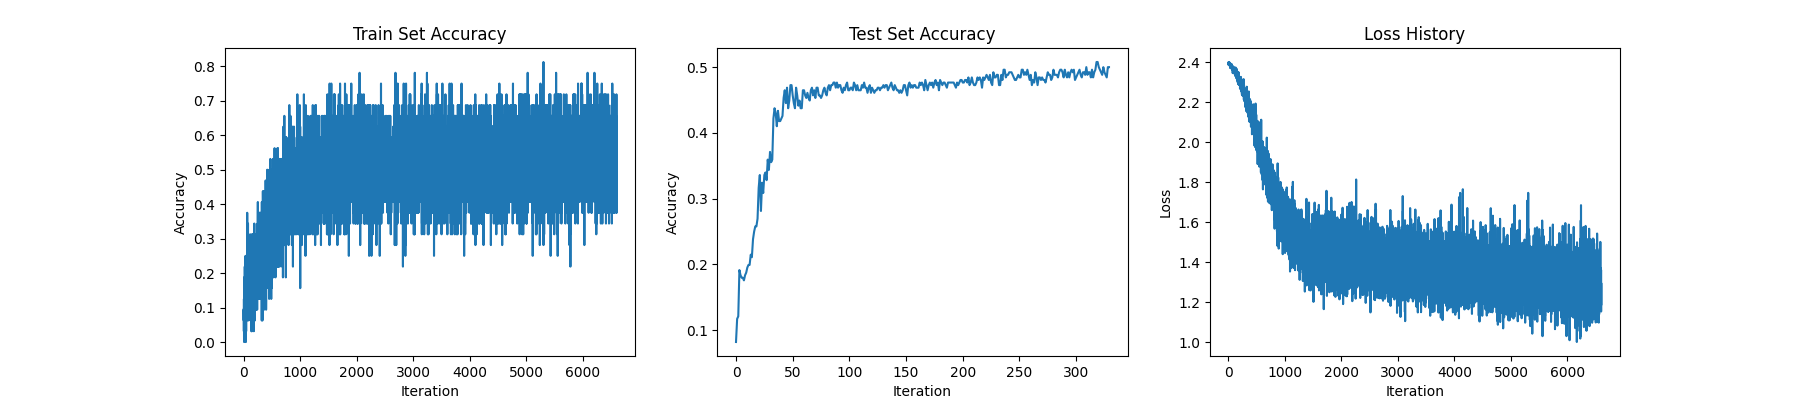
\includegraphics[width=\linewidth]{dvsgesture_dense_training.png}
    \caption{Dense SNN training on DVSGesture (200 epochs, $T=32$). Train accuracy reaches $\sim$70\%, test accuracy stabilizes near 50\%, and loss decreases steadily throughout training.}
    \label{fig:dvs_dense}
\end{figure}


\subsubsection{SHD}
Both SHD models train to near-perfect training accuracy but show a substantial gap on the test set (Figs.~\ref{fig:shd_dense}--\ref{fig:shd_sparse}). The dense model plateaus at $\sim$27\% test accuracy while the sparse model reaches $\sim$37\%, suggesting the spike regularization inadvertently acts as a form of regularization that improves generalization. Notably, the sparse model's loss increases over time—a consequence of the spike penalty growing as the model converges—while the dense model's loss decreases cleanly. Both curves motivate routing: neither model alone is clearly dominant.

\begin{figure}[H]
    \centering
    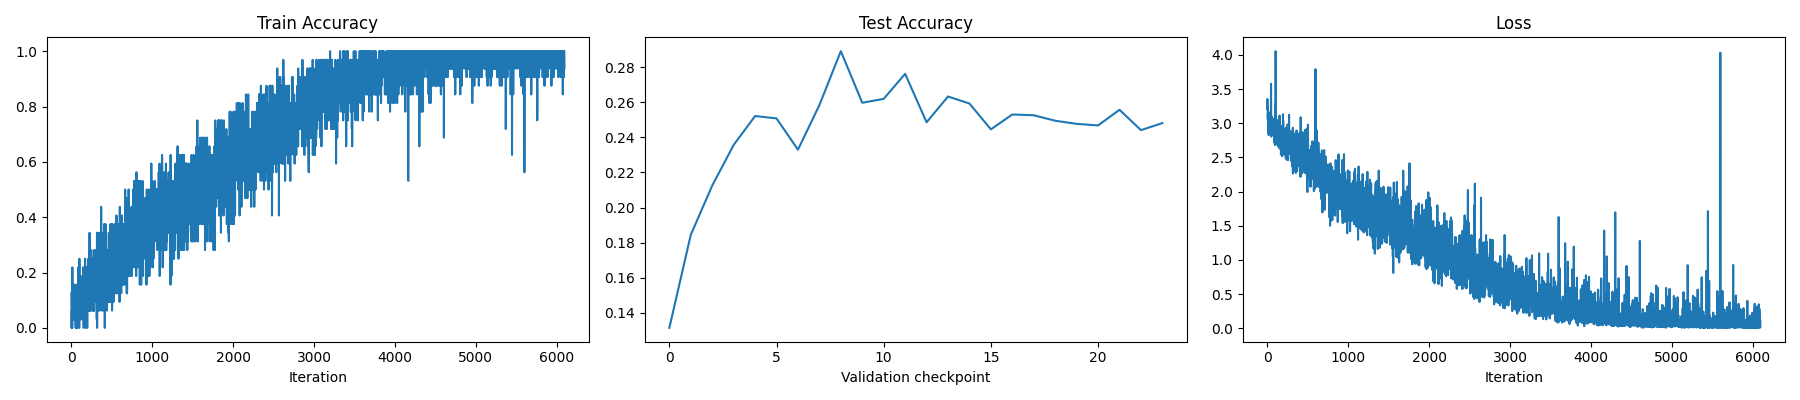
\includegraphics[width=\linewidth]{shd_dense_training.png}
    \caption{Dense SNN training on SHD. Training accuracy approaches 100\% while test accuracy plateaus near 25--28\%, indicating a significant generalization gap.}
    \label{fig:shd_dense}
\end{figure}

\begin{figure}[H]
    \centering
    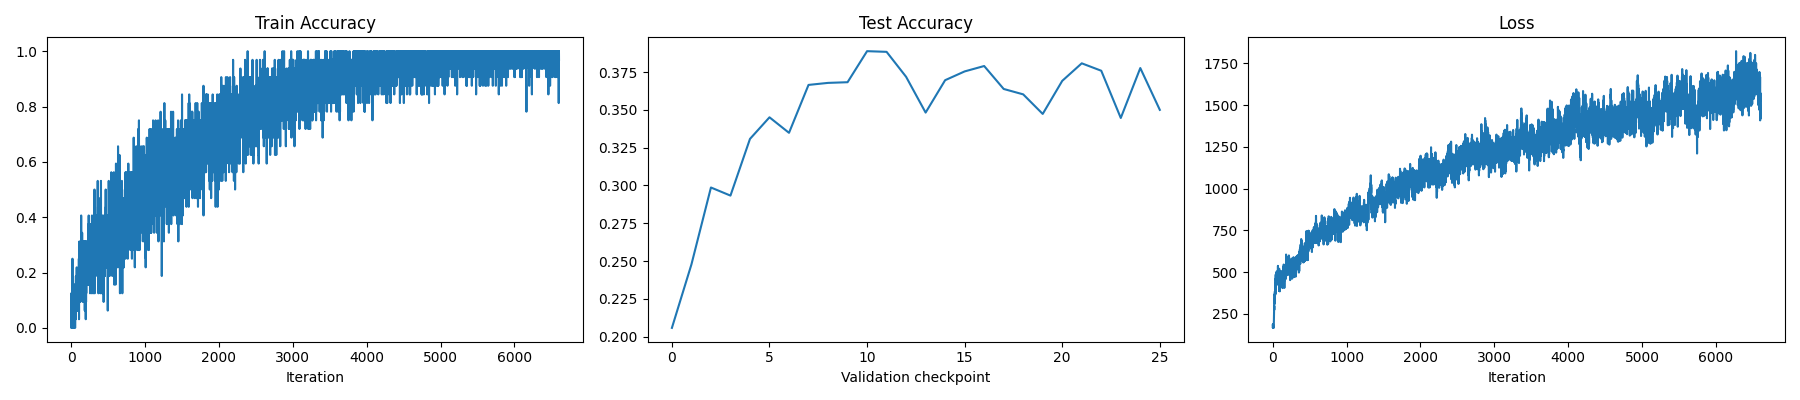
\includegraphics[width=\linewidth]{shd_sparse_training.png}
    \caption{Sparse SNN training on SHD. The model achieves similar training accuracy to the dense model but a higher test accuracy of $\sim$37\%, with loss increasing over time due to the spike regularization penalty.}
    \label{fig:shd_sparse}
\end{figure}


\subsubsection{UCI-HAR}
The UCI-HAR models converge quickly relative to the event-based datasets (Figs.~\ref{fig:uci_dense}--\ref{fig:uci_sparse}). The sparse model unexpectedly achieves higher test accuracy ($\sim$77\%) than the dense model ($\sim$70\%), which again likely reflects the regularizing effect of the spike penalty on this dataset. The smooth, continuous nature of IMU signals means spike activity does not vary dramatically between sparse and dense configurations, limiting the separation in firing rates between the two models.

\begin{figure}[H]
    \centering
    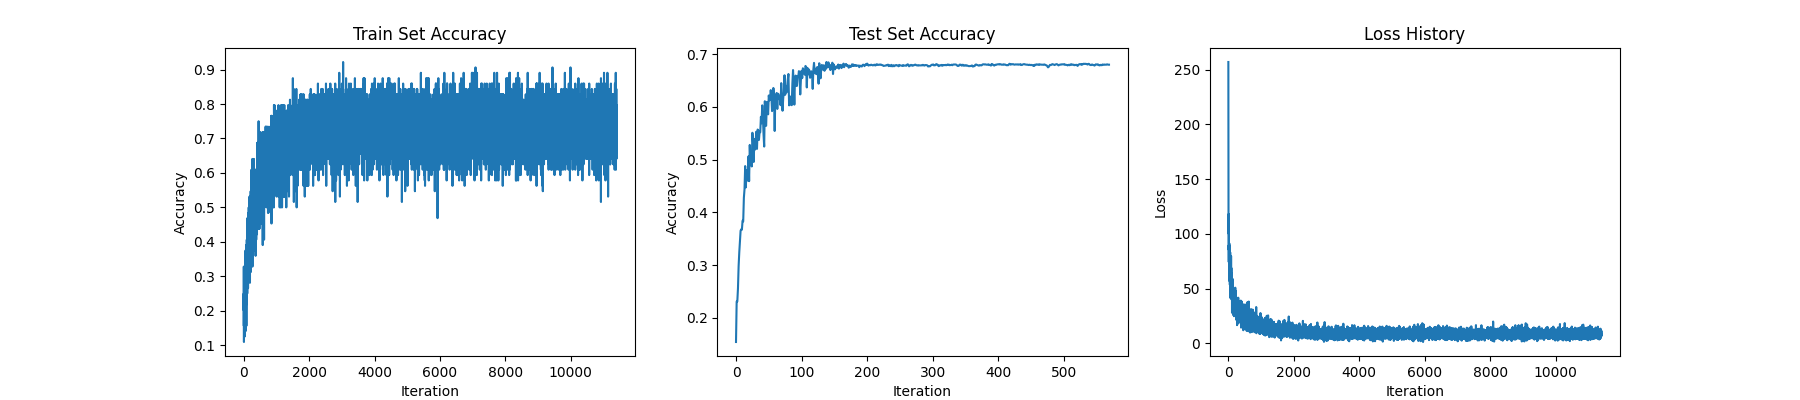
\includegraphics[width=\linewidth]{uci_har_dense_training.png}
    \caption{Dense SNN training on UCI-HAR (100 epochs, $T=128$). Test accuracy converges quickly to $\sim$70\% with a smooth loss curve.}
    \label{fig:uci_dense}
\end{figure}

\begin{figure}[H]
    \centering
    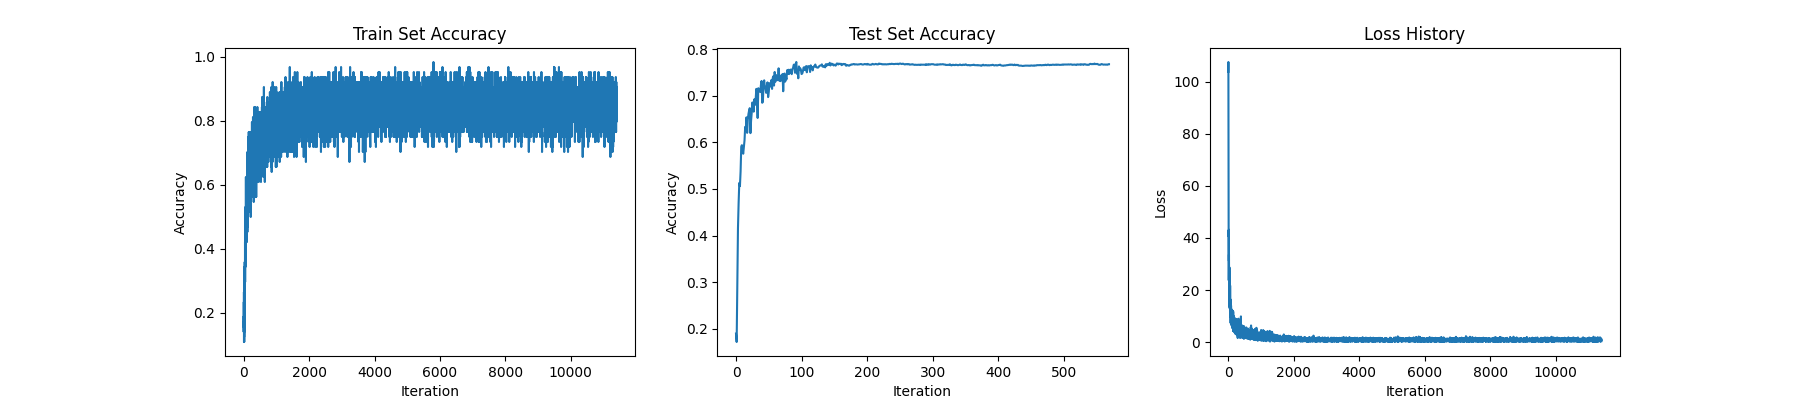
\includegraphics[width=\linewidth]{uci_har_sparse_training.png}
    \caption{Sparse SNN training on UCI-HAR. Test accuracy reaches $\sim$77\% with a slightly higher loss but smoother convergence than the dense model.}
    \label{fig:uci_sparse}
\end{figure}


\subsection{LZC Distributions and Routing Signal}

Across all three datasets, LZC shows a wide spread of values reflecting real variation in input complexity. DVSGesture samples range from $\sim$2000 to over 10{,}000, with the distribution showing a bimodal structure. Simpler gestures with repetitive motion patterns cluster at lower LZC values (2000--4000), while complex multi-directional gestures produce higher values. On SHD, LZC ranges from 19 to 75, and on UCI-HAR from 28 to 114. This spread across all datasets confirms that LZC captures meaningful variation in input structure that could support routing decisions.

\subsection{Router Energy: LZC on STM32}

\begin{figure}[H]
    \centering
    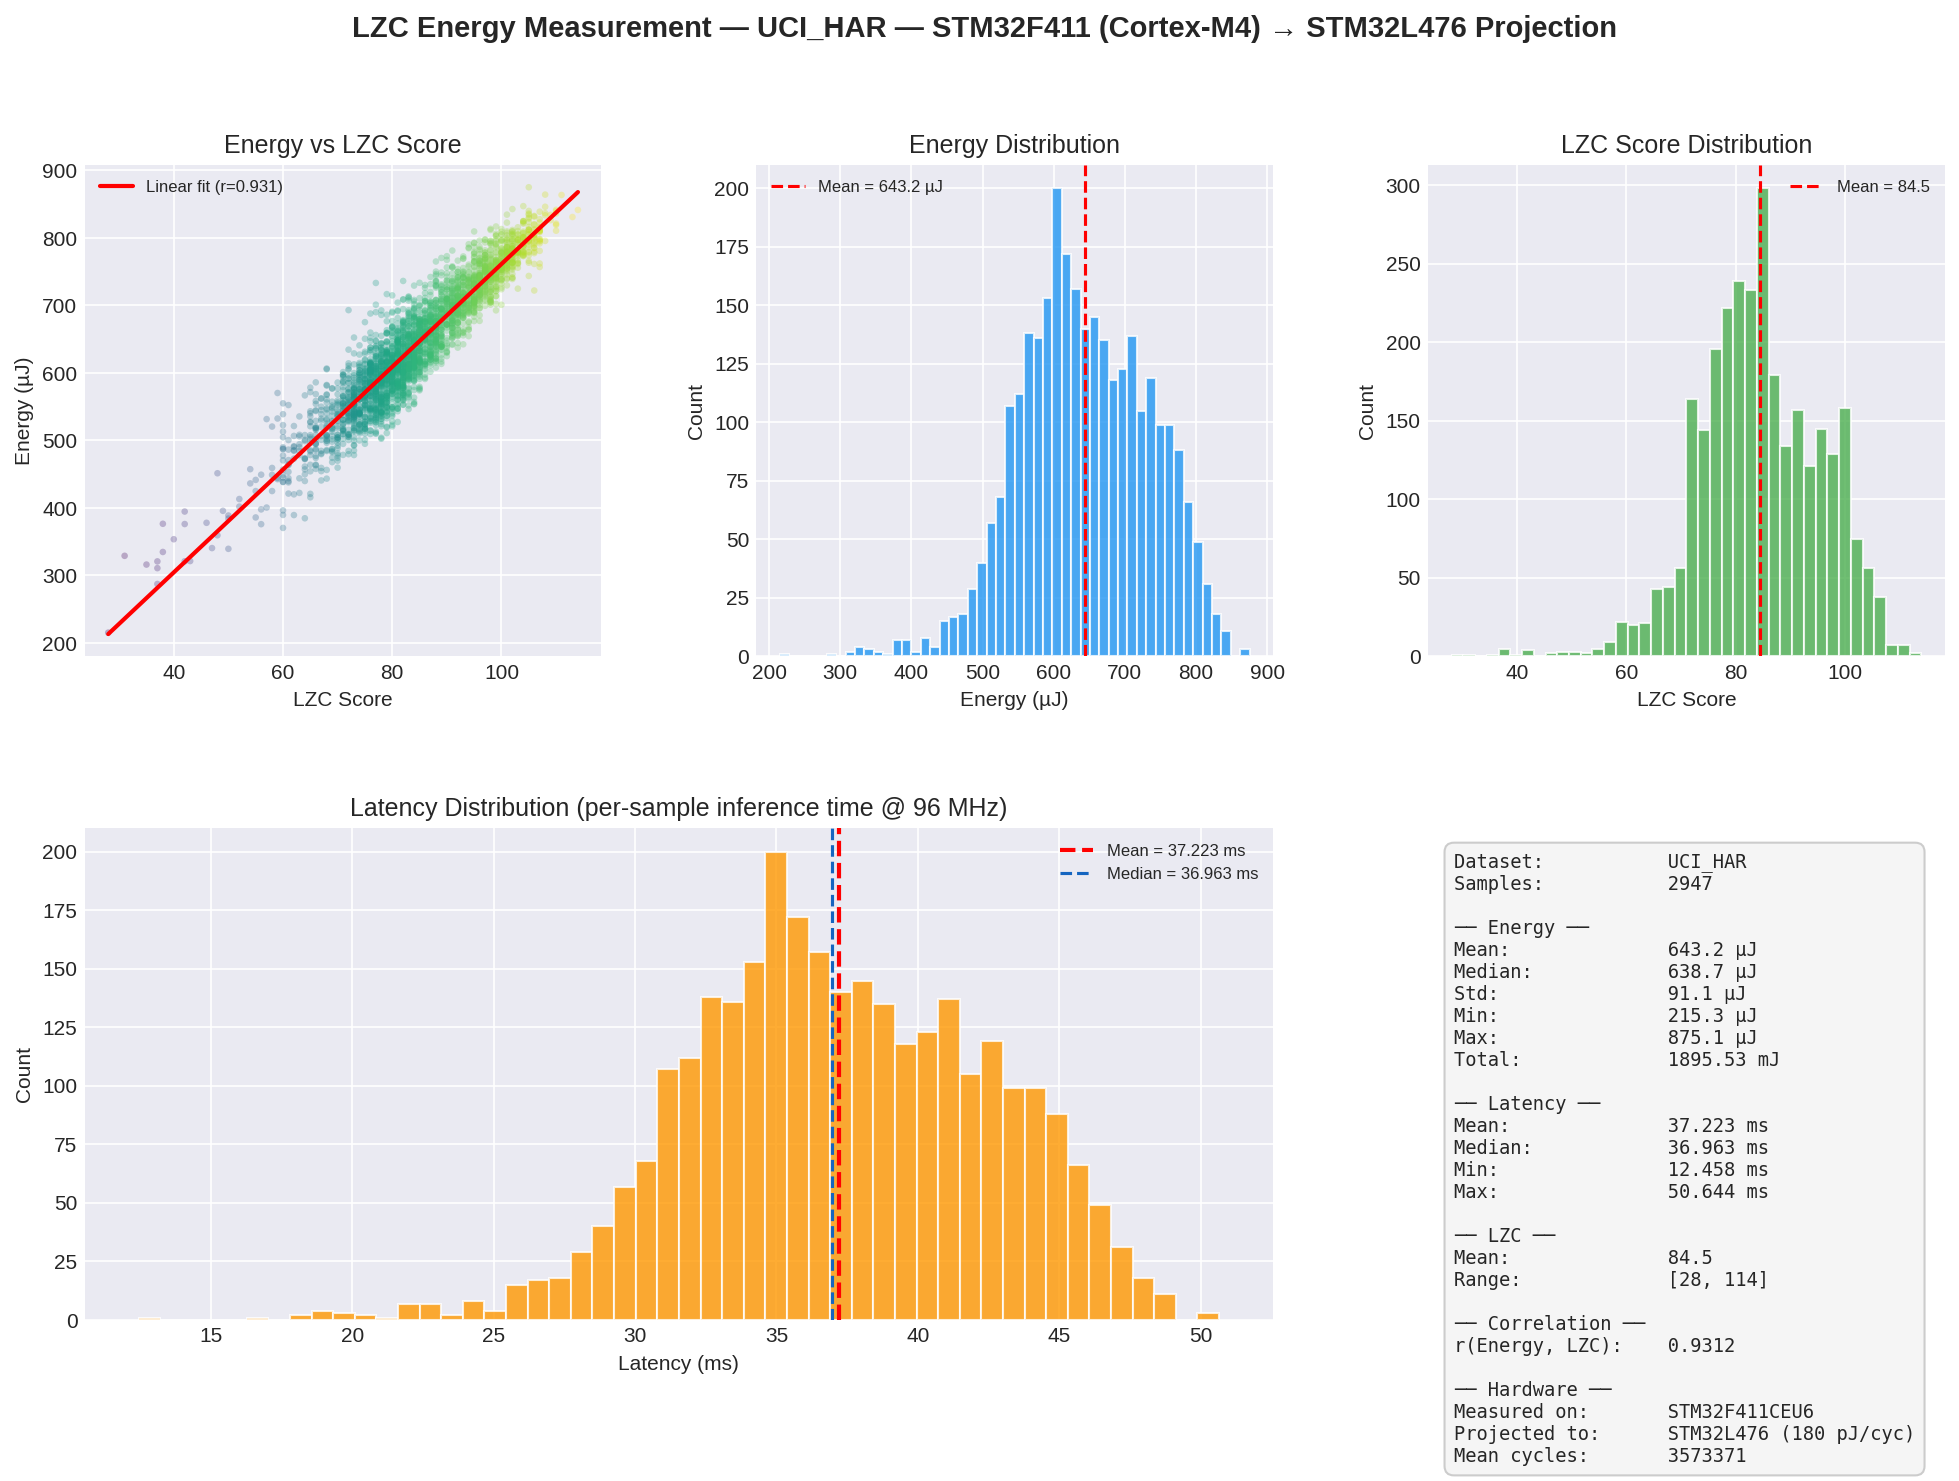
\includegraphics[width=\linewidth]{lzc_energy_plot_UCI_HAR.png}
    \caption{LZC energy and latency on UCI-HAR (2,947 samples). Mean energy: 643.2~$\mu$J, mean latency: 37.2~ms. The strong linear correlation ($r=0.931$) shows that more complex inputs take proportionally longer to score.}
    \label{fig:lzc_uci}
\end{figure}

\begin{figure}[H]
    \centering
    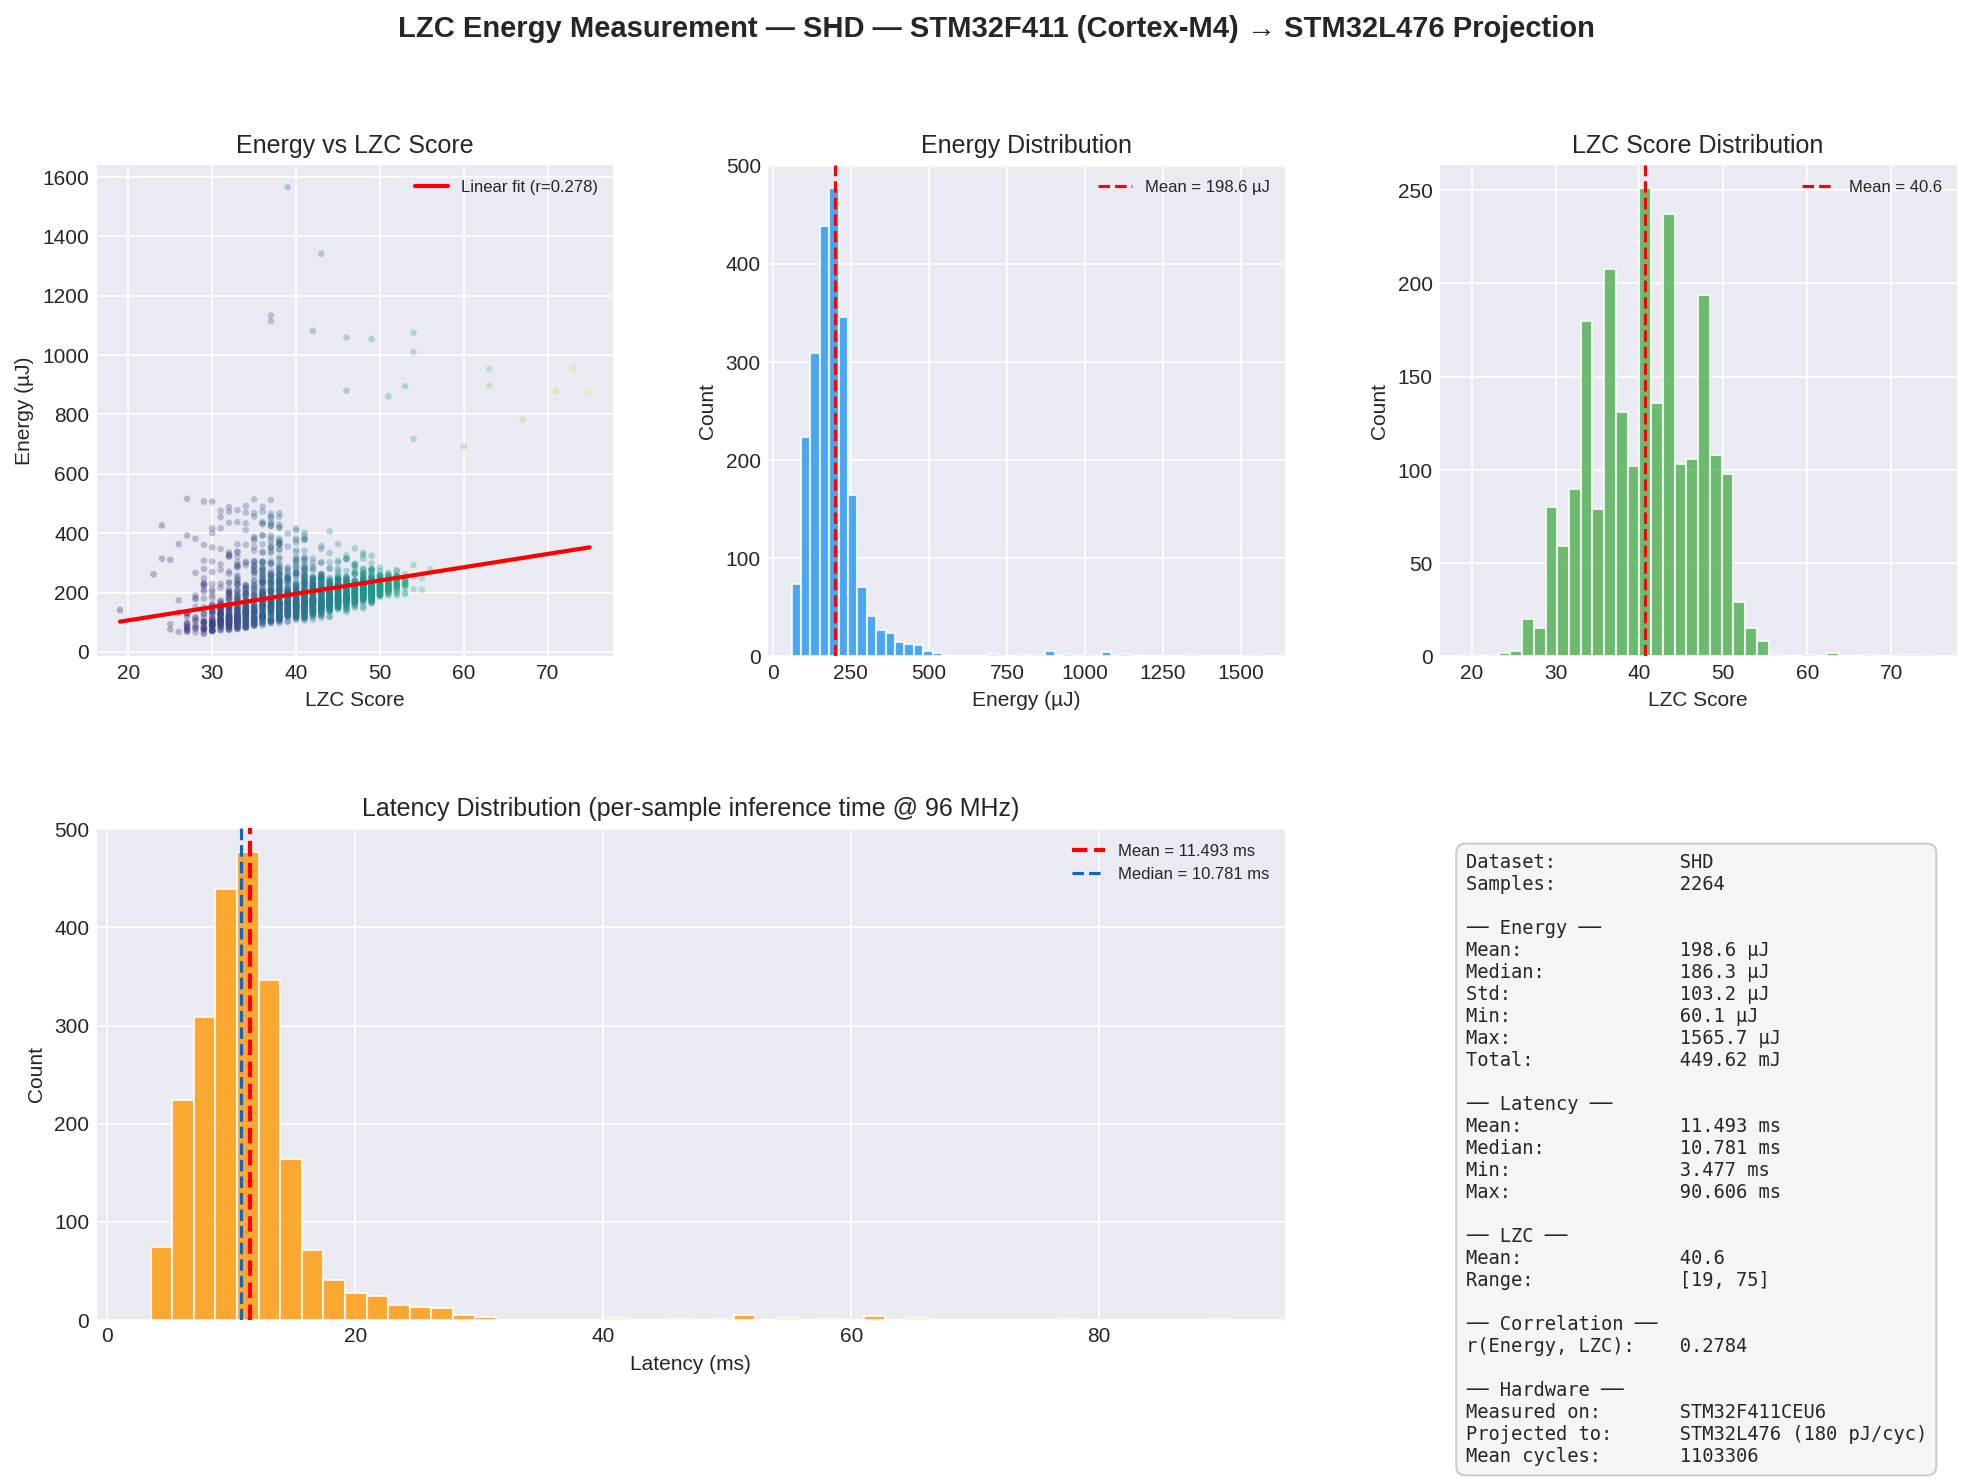
\includegraphics[width=\linewidth]{lzc_energy_plot_SHD.png}
    \caption{LZC energy and latency on SHD (2,264 samples). Mean energy: 198.6~$\mu$J, mean latency: 11.5~ms. The weaker correlation ($r=0.278$) reflects SHD's shorter, more uniform sequences.}
    \label{fig:lzc_shd}
\end{figure}

\begin{figure}[H]
    \centering
    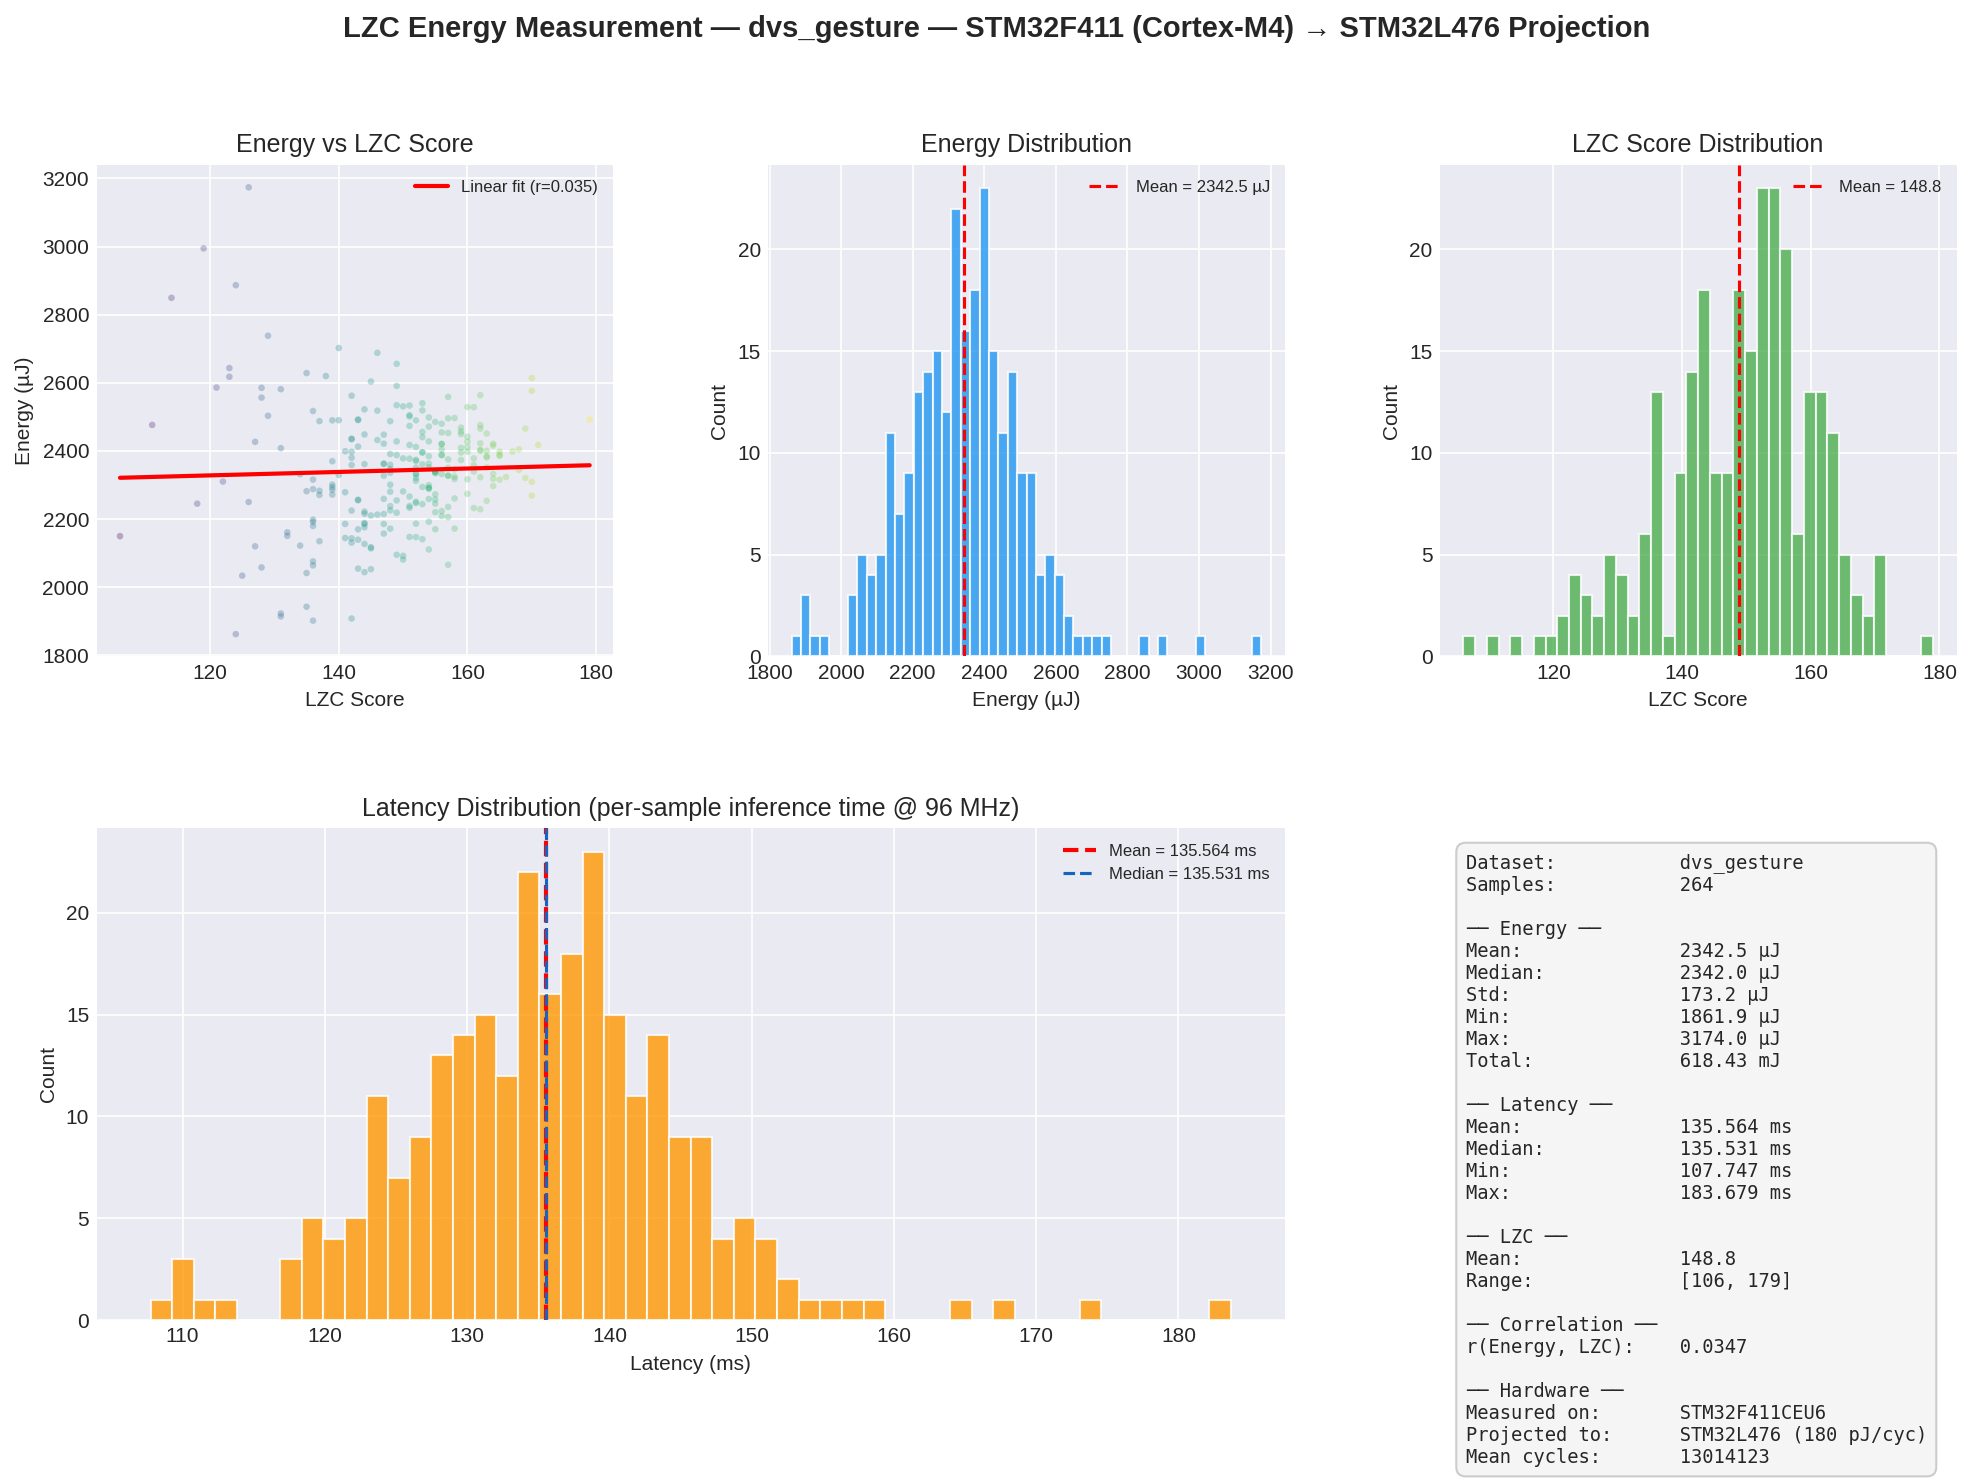
\includegraphics[width=\linewidth]{lzc_energy_plot_dvs_gesture.png}
    \caption{LZC energy and latency on DVSGesture (264 samples). Mean energy: 2,342.5~$\mu$J, mean latency: 135.6~ms. The negligible correlation ($r=0.035$) and very high cost make LZC impractical for this modality.}
    \label{fig:lzc_dvs}
\end{figure}

LZC computation costs are summarized in Table~\ref{tab:lzc_hw} and plotted in Figs.~\ref{fig:lzc_uci}--\ref{fig:lzc_dvs}. The results reveal a fundamental problem: LZC is expensive. On UCI-HAR, the mean energy is 643~$\mu$J per sample with a latency of 37~ms. On DVSGesture, whose samples flatten to a much longer binary string, mean energy reaches 2,342~$\mu$J and latency 136~ms. These costs exceed the SNN inference energy on Xylo by orders of magnitude, making LZC routing counterproductive from an energy standpoint.

\begin{table}[H]
\centering
\caption{LZC hardware energy and latency (STM32L476 projection).}
\label{tab:lzc_hw}
\begin{tabular}{lcccr}
\toprule
\textbf{Dataset} & \textbf{N} & \textbf{Energy ($\mu$J)} & \textbf{Latency (ms)} & \textbf{$r$} \\
\midrule
UCI-HAR     & 2,947 & 643.2  & 37.22  & 0.931 \\
SHD         & 2,264 & 198.6  & 11.49  & 0.278 \\
DVSGesture  &   264 & 2342.5 & 135.56 & 0.035 \\
\bottomrule
\end{tabular}
\end{table}

\subsection{Router Energy: Transition Count on STM32}

\begin{figure}[H]
    \centering
    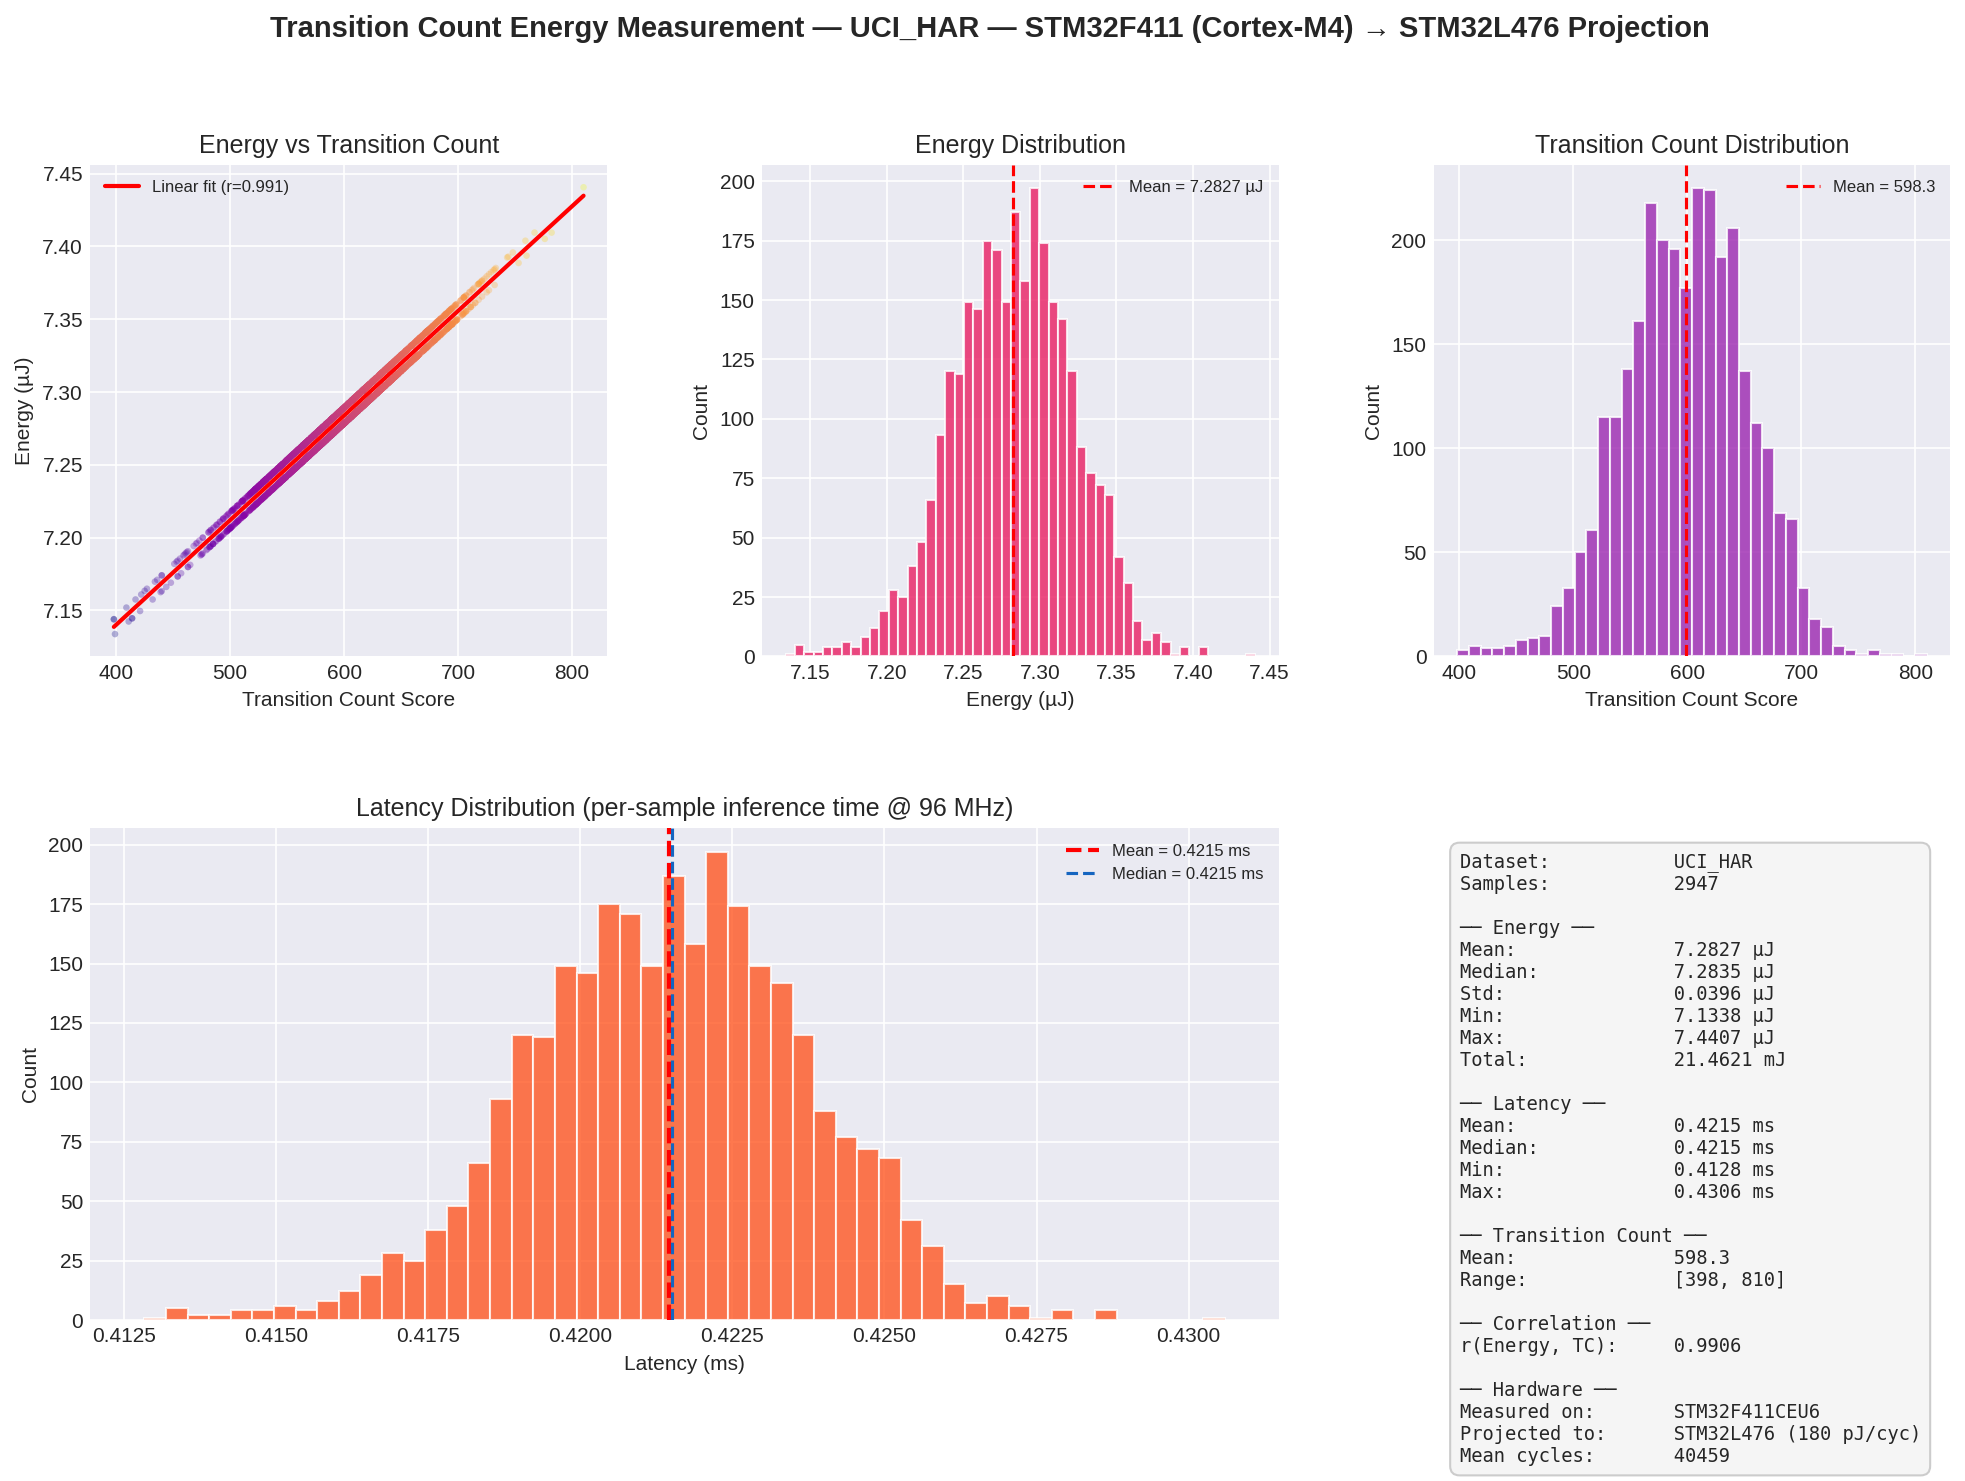
\includegraphics[width=\linewidth]{tc_energy_plot_UCI_HAR.png}
    \caption{TC energy and latency on UCI-HAR (2,947 samples). Mean energy: 7.28~$\mu$J, mean latency: 0.42~ms. TC is \textbf{88$\times$} cheaper than LZC on this dataset with a near-perfect complexity correlation ($r=0.991$).}
    \label{fig:tc_uci}
\end{figure}

\begin{figure}[H]
    \centering
    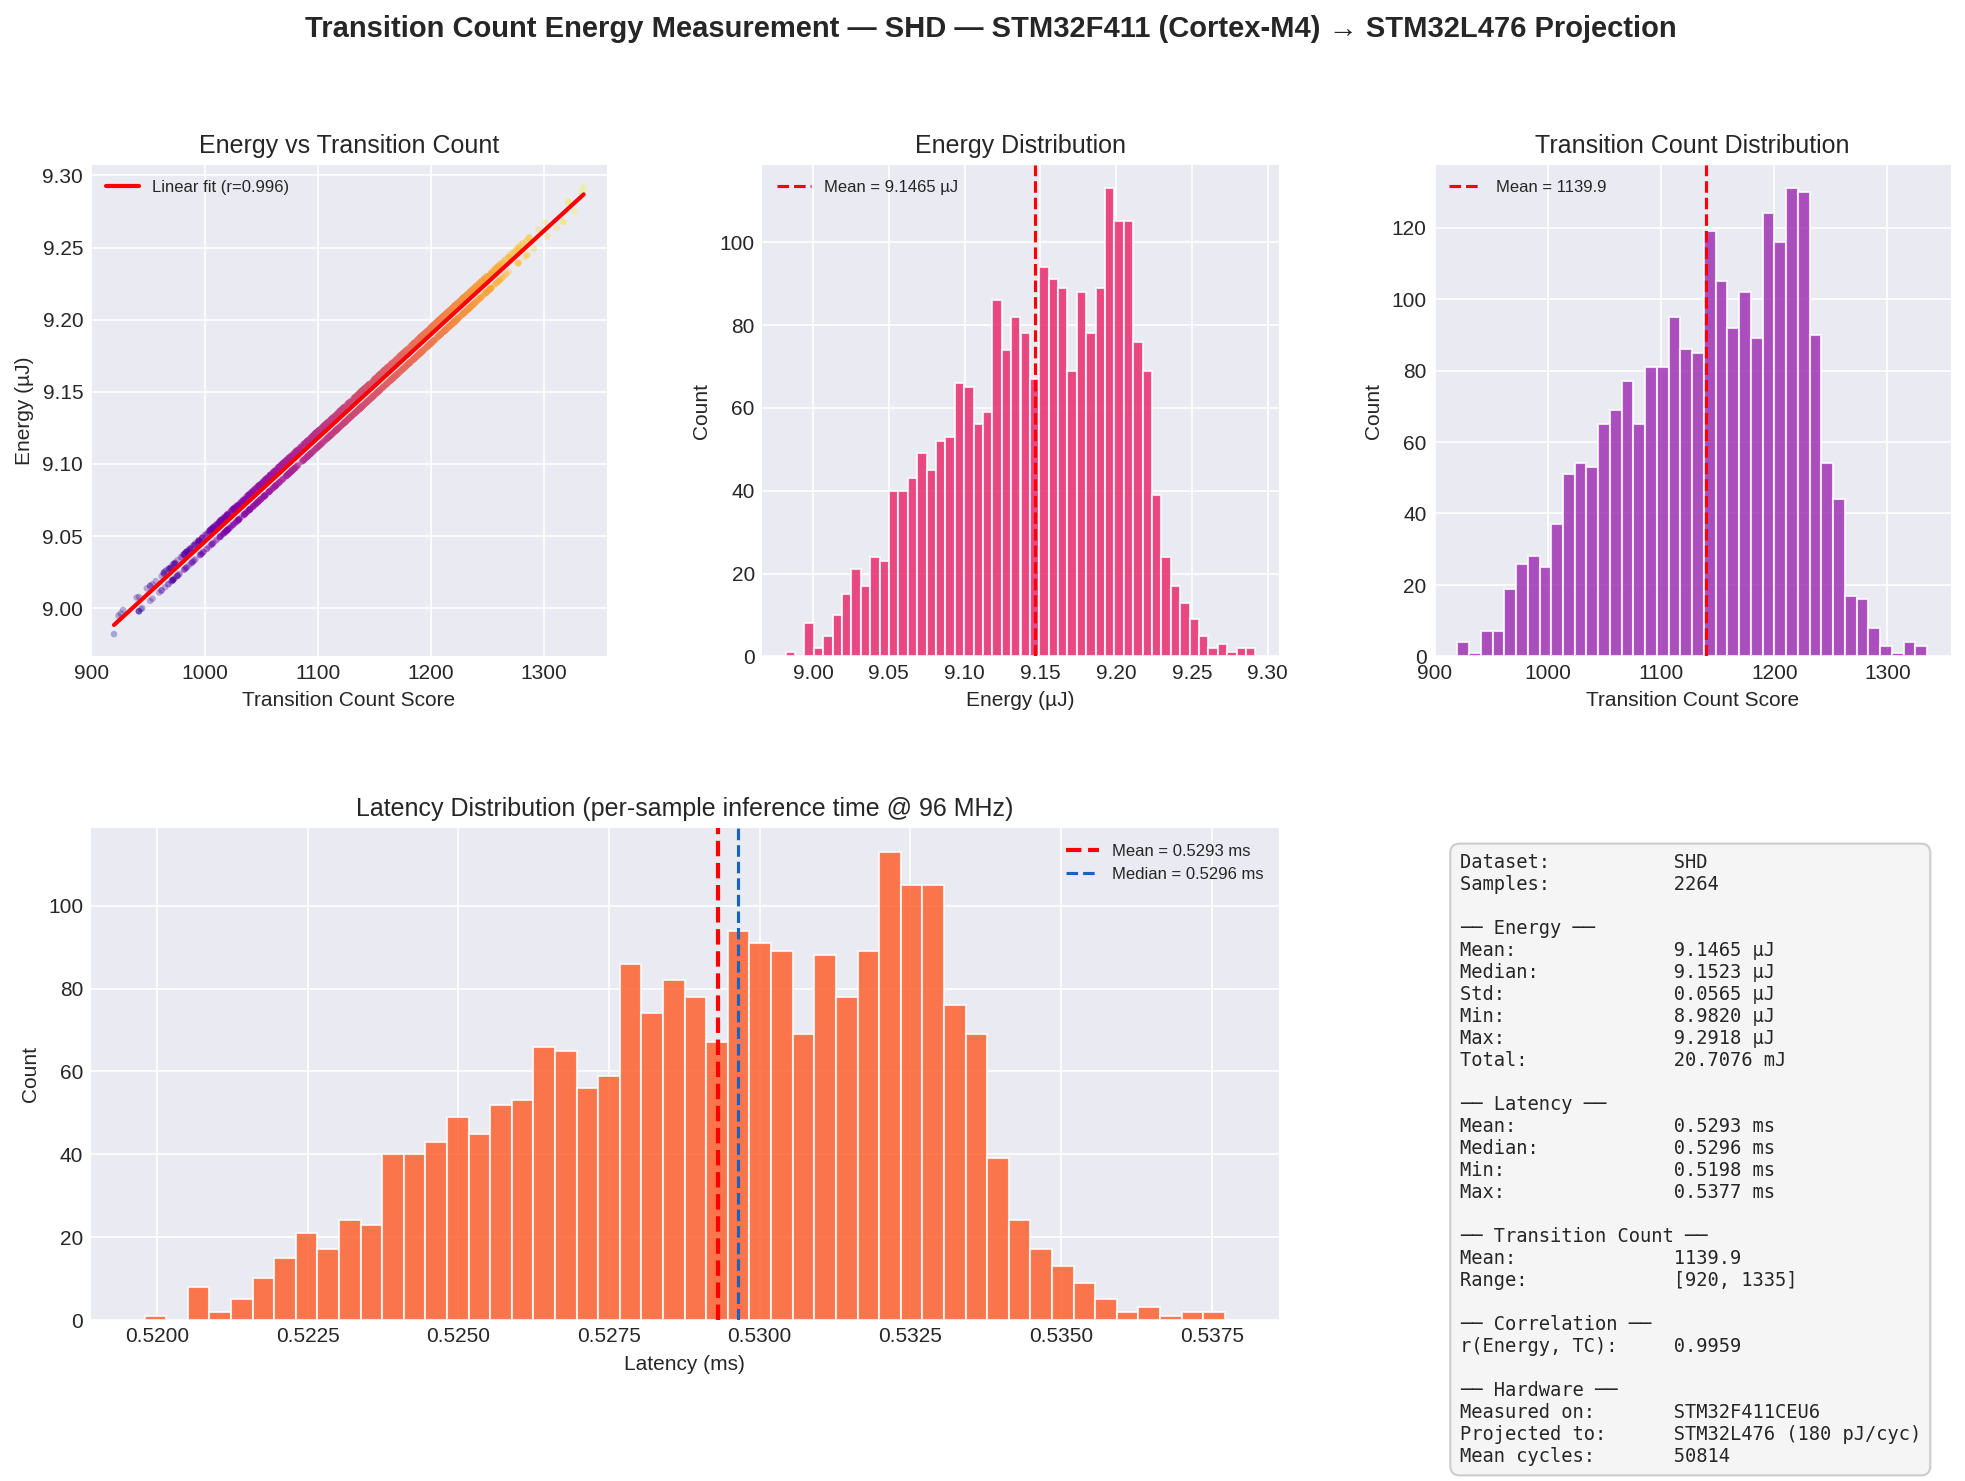
\includegraphics[width=\linewidth]{tc_energy_plot_SHD.png}
    \caption{TC energy and latency on SHD (2,264 samples). Mean energy: 9.15~$\mu$J, mean latency: 0.53~ms. TC is \textbf{22$\times$} cheaper than LZC while achieving a stronger correlation ($r=0.996$).}
    \label{fig:tc_shd}
\end{figure}

\begin{table}[H]
\centering
\caption{TC hardware energy and latency (STM32L476 projection).}
\label{tab:tc_hw}
\begin{tabular}{lcccr}
\toprule
\textbf{Dataset} & \textbf{N} & \textbf{Energy ($\mu$J)} & \textbf{Latency (ms)} & \textbf{$r$} \\
\midrule
UCI-HAR & 2,947 & 7.28 & 0.421 & 0.991 \\
SHD     & 2,264 & 9.15 & 0.529 & 0.996 \\
\bottomrule
\end{tabular}
\end{table}

TC results are shown in Figs.~\ref{fig:tc_uci}--\ref{fig:tc_shd} and Table~\ref{tab:tc_hw}. The contrast with LZC is stark. TC costs only 7.28~$\mu$J per sample on UCI-HAR (0.42~ms latency) and 9.15~$\mu$J on SHD (0.53~ms)—reductions of 88$\times$ and 22$\times$, respectively. TC's latency is also nearly constant across samples (0.41--0.43~ms on UCI-HAR), compared to LZC's 4$\times$ range (12.5--50.6~ms), because TC's linear scan has no data-dependent branching. Critically, TC achieves \emph{higher} complexity correlation than LZC on both datasets ($r > 0.99$), meaning it is not just faster—it is also a more consistent routing signal.

\begin{table}[H]
\centering
\caption{LZC vs.\ TC: energy and correlation comparison.}
\label{tab:lzc_vs_tc}
\begin{tabular}{llccr}
\toprule
\textbf{Dataset} & \textbf{Metric} & \textbf{Energy ($\mu$J)} & \textbf{Latency (ms)} & \textbf{$r$} \\
\midrule
UCI-HAR & LZC & 643.2 & 37.22 & 0.931 \\
UCI-HAR & TC  & 7.28  & 0.421 & 0.991 \\
\midrule
SHD     & LZC & 198.6 & 11.49 & 0.278 \\
SHD     & TC  & 9.15  & 0.529 & 0.996 \\
\bottomrule
\end{tabular}
\end{table}

\subsection{Entropy Threshold Optimization}

\begin{figure}[H]
    \centering
    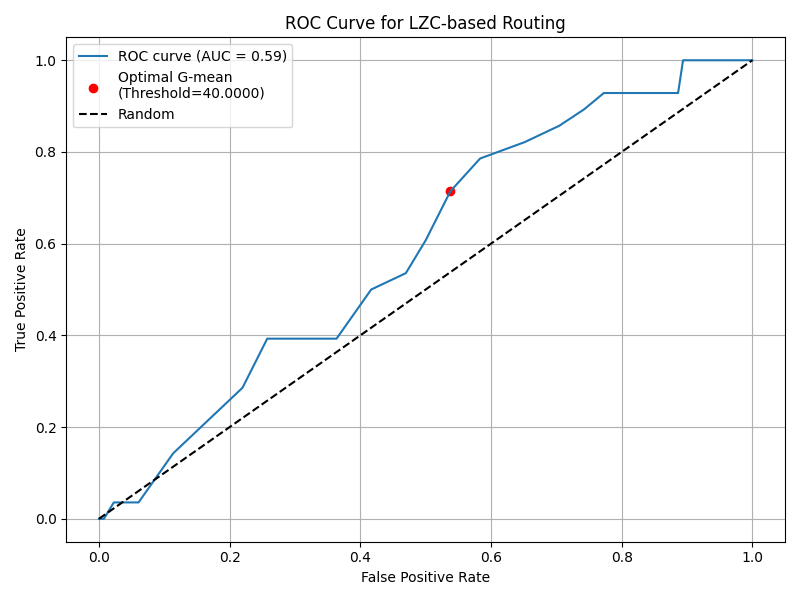
\includegraphics[width=\linewidth]{roc_shd.png}
    \caption{ROC curve for LZC-based routing on SHD. AUC = 0.59; the optimal G-mean threshold is 40.0. The curve sits above the random baseline, confirming LZC contains a usable routing signal despite its high compute cost.}
    \label{fig:roc_shd}
\end{figure}

Fig.~\ref{fig:roc_shd} shows the ROC curve for LZC-based routing on SHD. The AUC of 0.59 is modest but above chance, confirming that LZC contains a usable—if weak—routing signal. The G-mean-optimal threshold of 40.0 balances sensitivity and specificity, routing 57\% of samples to the sparse model and 43\% to the dense model. The smooth variation of performance across thresholds supports systematic threshold selection via G-mean optimization.

\subsection{End-to-End Routing Results}

\begin{table}[H]
\centering
\caption{DVSGesture routing performance and spike activity.}
\label{tab:routing}
\begin{tabular}{lc}
\toprule
Metric & Value \\
\midrule
Optimal LZC threshold & 6094 \\
ROC-AUC               & 0.585 \\
Overall accuracy      & 0.784 \\
Dense-route accuracy  & 0.893 \\
Sparse-route accuracy & 0.714 \\
Avg dense spikes      & 31,220 \\
Avg sparse spikes     & 2,567 \\
Samples to dense      & 103 \\
Samples to sparse     & 161 \\
\bottomrule
\end{tabular}
\end{table}

Table~\ref{tab:routing} shows routing results on DVSGesture. Using the G-mean-optimal threshold of 6094, the routed system achieves an overall accuracy of 78.4\%. Samples routed to the dense model reach 89.3\% accuracy, while sparse-routed samples achieve 71.4\%. Critically, the sparse route produces an average of 2,567 spikes per sample compared to 31,220 for the dense route—a 12$\times$ reduction in spike activity and corresponding energy savings \emph{at the SNN level}.

However, when router energy is included, the picture changes. The dense SNN consumes approximately $4.09\times10^{-6}$~J per sample and the sparse SNN $2.50\times10^{-7}$~J, while LZC routing on the STM32 costs approximately $5.00\times10^{-4}$~J per sample. The router dominates the energy budget by more than two orders of magnitude, resulting in net negative energy savings of $-15{,}973\%$ relative to always using the dense model. Routing with LZC does not reduce total system energy in this configuration.

\subsection{Xylo Inference Energy and Latency Results}

\begin{table}[H]
\centering
\caption{Xylo-measured routing performance on UCI HAR.}
\label{tab:xylo}
\begin{tabular}{lc}
\toprule
Metric & Value \\
\midrule
Optimal LZC threshold & 191 \\ % TEMPORARY NUMBERS; DON'T WORRY FOR NOW vvvvvvvv
ROC-AUC               & 0.387 \\
Overall accuracy      & 0.21 \\ 
Dense-route accuracy  & 0.111 \\ 
Sparse-route accuracy & 0.174 \\ 
Avg dense spikes      & 33,286 \\
Avg sparse spikes     & 7,933 \\
Avg dense inference time      & 9.534 \\
Avg sparse inference time     & 9.536 \\
Samples to dense      & 27 \\
Samples to sparse     & 73 \\
\bottomrule
\end{tabular}
\end{table}

Table~\ref{tab:xylo} shows routing results on UCI HAR. Similarly to the previous subsection, the sparse SNN produces much less spikes than the dense SNN, this time at a 4$\times$ reduction in spike activity.

Including LZC costs, the dense SNN consumes approximately $3.26\times10^{-2}$~J per sample, and the sparse SNN $3.25\times10^{-2}$~J. LZC computation contributes approximately 2\% of the total energy per SNN. The router is able to remain effectively negligible while resulting in energy savings of $0.12\%$ relative to always using the dense model. As opposed to using the STM32, routing with LZC reduces total system energy in this configuration.

Excluding latency from the LZC computation, the average latency per inference was 9.53 seconds for both the sparse and dense model. LZC computation adds $4.54\times10^{-2}$~ seconds for the sparse model and $5.08\times10^{-2}$~ seconds for the dense model. The total runtime, including LZC routing, was 953.5 seconds over the evaluated sample set. Therefore, LZC routing made up for about 0.48\% of the total inference time for the sparse model, and 0.53\% for the dense model. These measurements show that while Xylo provides low-energy inference, sample-level latency remains substantial under the current sequential evaluation setup.

The measured Xylo inference times also provide an important reference point for interpreting the routing results. Even when routing selects the more efficient model, the end-to-end runtime is dominated by hardware inference latency rather than the complexity metric itself. This makes throughput an additional practical limitation alongside energy consumption.

\subsection{ANN-Based Router Results}

A preliminary ANN router was trained to predict model selection from extracted features (LZC score, spike count, standard deviation, and other temporal statistics). The resulting ROC curve yields an AUC of approximately 0.59—similar to the entropy-based router. The ANN's performance was limited by the small size of the DVSGesture dataset (1,077 training samples), potential feature under-expressiveness, and class imbalance. These results are treated as a baseline for future development rather than a primary finding.

% ---------------------------------------------------------------
\section{Discussion and Conclusion}
% ---------------------------------------------------------------

\subsection{Key Findings}

Our results confirm two things simultaneously. First, there is real efficiency potential in routing: the sparse SNN produces 12$\times$ fewer spikes than the dense model on DVSGesture, and routing correctly identifies many inputs that can be handled by the sparse model without sacrificing accuracy. Second, the current LZC-based router costs far more energy to run than it saves. This is not a failure of the routing concept—it is a failure of LZC as a routing signal for embedded deployment.

The hardware measurements make this concrete. LZC costs 643~$\mu$J per sample on UCI-HAR and 2,342~$\mu$J on DVSGesture, compared to SNN inference costs on the order of $10^{-6}$~J per sample on Xylo. TC reduces this to 7--9~$\mu$J while improving the complexity correlation from $r = 0.28$--$0.93$ (LZC) to $r > 0.99$ (TC). TC is not only cheaper—it is a more reliable measure of the input structure relevant for routing.

The Xylo measurements sharpen the interpretation of our results. Our routing system is not only an energy problem but also a systems problem: a routing signal may still be impractical if the inference is excessively long. In our current setup, Xylo inference time is the dominant runtime cost, while routing overhead is comparatively small but still non-negligible in energy terms. This suggests that future routing methods should not be evaluated only by classification accuracy or routing quality, but also by their compatibility with deployment constraints such as per-sample inference latency, batching support, and on-chip execution.

\subsection{Implications for Neuromorphic Routing}

These findings point to a broader design principle: for routing to produce net energy savings on neuromorphic hardware, the routing mechanism itself must be nearly free. SNN inference at the speeds enabled by hardware like Xylo is already extremely cheap, and any CPU-side computation can easily erase that advantage. Effective routing signals should be simple, predictable, and ideally computable from early spike statistics before the full input is processed—or implemented directly on-chip.

TC is a step in this direction. Its linear-time structure and near-zero branching make it a candidate for on-chip implementation in future neuromorphic architectures. LZC, by contrast, requires a growing dictionary of seen patterns and has data-dependent execution time, making it poorly suited to the deterministic, low-power compute environment of a neuromorphic chip.

\subsection{Limitations}

The primary limitation is that neither LZC nor TC currently produces net energy savings when routing overhead is included. Both metrics are still computed on a CPU rather than on-chip. LZC is clearly not viable; TC is promising but not yet sufficient. Additionally, the sparse and dense SNN variants on UCI-HAR show limited firing rate separation, likely because IMU signals are smoother and more continuous than event-based data and do not benefit as strongly from spike suppression. Further parameter tuning or alternative neuron models may improve this.

An additional limitation is that our Xylo inference measurements were obtained under a sequential evaluation setup, so the reported latency reflects per-sample runtime rather than amortized batch output. This is appropriate for edge deployment analysis, but it means the results should be interpreted as a conservative estimate of runtime cost.

The ANN router remains preliminary and requires larger datasets and more expressive features to be competitive.

\subsection{Future Work}
The most impactful next step is investigating whether TC or similar linear-scan metrics can be implemented on neuromorphic hardware or approximated from partial spike observations before the full input arrives. Multi-stage routing—using a cheap early estimate to decide whether to continue processing—is another promising direction. On the model side, exploring intermediate configurations between fully sparse and fully dense could allow finer-grained routing with better energy-accuracy tradeoffs. 

Future work should also explore on-chip or partially on-chip routing to eliminate CPU-side complexity computation, as well as output improvements through batching, pipelining, or early-exit inference. Another promising direction is to redesign the SNNs and routing metric jointly so that routing cost, inference latency, and model accuracy are optimized together at deployment time.

Finally, hardware deployment of the SHD model on Xylo would enable direct measurement of spike activity, latency, and energy for the neuromorphic audio use case.

\subsection{Conclusion}

This work demonstrates both the potential and the current limitations of entropy-based routing for energy-efficient SNNs. Sparse SNNs produce substantially fewer spikes than dense ones, and complexity-based routing can effectively direct simple inputs to the cheaper model. However, our hardware measurements show that LZC routing is not viable at the embedded scale: it costs hundreds to thousands of $\mu$J per sample while SNN inference costs only $\mu$J or less on Xylo. Transition Count offers an 88$\times$ energy reduction over LZC while improving routing correlation—a meaningful step toward a practical routing signal. The core finding is a design principle: for neuromorphic routing to pay off, the routing mechanism must be as lightweight as the inference it governs.

\section*{Acknowledgment}
The initial concept for this work was proposed by Gaurav Gupta. All authors contributed substantially to the design, implementation, analysis, and writing of this study. The supervising faculty member is listed last.

\printbibliography
\end{document}